\section{Knowledge formalization}
\label{sec:tkm:k-formalism}
 
  As discussed previously, I consider \gls{knowledge} to be the association of \gls{context} information, \glspl{requirement}, and \gls{action} information, all in one global and unified model.
 While \gls{context} information captures the state of the system environment and its surroundings, the system \glspl{requirement} define the constraints that the system should satisfy along the way. 
 The \glspl{action}, on the other hand, are means to reach the goals of the system.
  
 In this section, I provide a formalization of the \gls{knowledge} used by adaptation processes based on a temporal graph. 
Indeed, due to the complexity and interconnectivity of system entities, graph data representation seems to be an appropriate way to represent the \gls{knowledge}. 
Augmented with a temporal dimension, temporal graphs are then able to symbolize the evolution of system entities and states over time. 
We benefit from the well-defined graph manipulation operations, namely temporal graph pattern matching and temporal graph relations to represent the traceability links between the \glspl{decision} made and their \glspl{circumstance}.

Before describing this formalism, I describe the semantic used for the temporal axis.
Then, I exemplify the knowledge formalism using the Luxembourg smart grid use case.

\subsection{Formalization of the temporal axis}
\label{sec:tkm:timeDef}

\begin{figure}
   \centering
	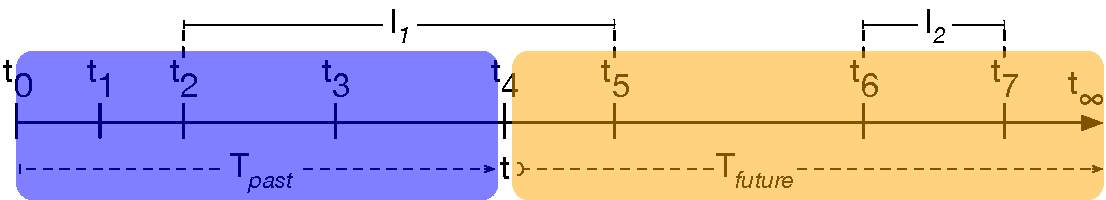
\includegraphics[width=\textwidth]{img/chapt-tkm/formalism/formalismeTime}
	\caption{Time definition used for the knowledge formalism}
	\label{fig:tkm:formalismeTime}
\end{figure}

The formalism describe below has been made with two goals in mind.
First, the definition of the time space should allow the distinction between past and future. 
Doing this distinction enable the differentiation between measured data and estimated (or predicted data).
Second, it should permit the definition of the life cycle of an element of the \gls{knowledge}, which can be seen as a succession of states with a validity period that should not overlap each other.

Time space $T$ is considered as an ordered discrete set of time points non-uniformly distributed. 
As depicted in Figure~\ref{fig:tkm:formalismeTime}, this set can be divided into 3 different subsets $T = T_{past} \cup \{t\} \cup T_{future}$, where:  
\begin{itemize}
	\item $T_{past}$ is the sub-domain \{$t_{0}$;$t_{1}$;\ldots;$t_{current-1}$\}  representing graph data history starting from $t_0$, the oldest point, until current time, t, excluded.
	\item \{t\} is a singleton representing the current time 
point
	\item $T_{future}$ is sub-domain \{$t_{current+1};\ldots;t_{\infty}$\} representing future time points 
\end{itemize}
The three domains depend completely on the current time \{t\} as these subsets slide as time passes. 
At any point in time, these domains never overlap: $T_{past} \cap \{t\} = \emptyset$, $T_{future} \cap \{t\} =  \emptyset$, and $T_{past} \cap T_{future} = \emptyset$.
The definition of these three subsets reachs the first goal.

In addition, there is a right-opened time interval $I \in T \times T$ as $[t_s, t_e)$ where $t_e - t_s > 0$.
In English words, it means that the interval cannot represent a single time point and should follow the time order. 
For any $i \in I$, $start(i)$ denotes its lower bound and $end(i)$ its upper bound.
As detailed in Section~\ref{sec:tkm:formalism}, these intervals are used to define the validity period for each node of the graph. 

Figure~\ref{fig:tkm:formalismeTime} displays an example of a time space $T_1 = \{t_0, t_1, t_2, t_3, t_4, t_5, t_6, t_7\}$.
Here, the current time is $t = t_4$.
According to the definition of the past subset ($T_{past}$) and the future one ($T_{future}$), there is: $T_{past1} =  \{t_0, t_1, t_2, t_3\}$ and $T_{future1} = \{t_5, t_6, t_7\}$.
Two intervals have been defined on $T_1$, namely $I_1$ and $I_2$.
The first one starts at $t_2$ and ends at $t_5$ and the last one is defined from $t_6$ to $t_7$.
As shown with $I_1$, an interval could be defined on different subsets, here it is on all of them ($T_{past}$, $t$, and $T_{future}$).

\subsection{Formalism}
\label{sec:tkm:k-formalism:formalism}
 
\paragraph{Graph definition}
First, let $K$ be an adaptive process over a system \gls{knowledge} represented by a graph such as $K = (N, E)$, comprising a set of nodes $N$ and a set of edges $E$.
Nodes represent any element of the knowledge (context, actions, \etc) and edges represent their relationships.
Nodes have a set of attribute values.
An attribute value has a type (numerical, boolean, \ldots). 
Every relationship $e \in E$ can be considered as a couple of nodes $(n_s, n_t) \in N \times N$, where $n_s$ is the source node and $n_t$ is the target node.

\paragraph{Adding the temporal dimension}

\begin{figure}
   \centering
	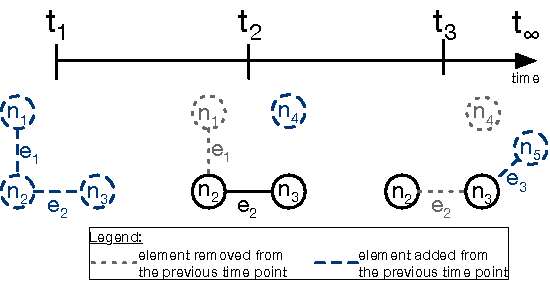
\includegraphics{img/chapt-tkm/formalism/validityExample}
	\caption{Evolution of a temporal graph over time}
	\label{fig:tkm:validityEx}
\end{figure}

In order to augment the graph with a temporal dimension, the relation $V^T$ is added.
So now the knowledge $K$ is defined as a temporal graph such as $K = (N, E, V^T)$.

A node is considered valid either until it is removed or until one of its attributes value changes. 
In the latter case, a new node with the updated value is created.
Whilst, an edge is considered valid until either its source node and target node is valid, or until the edge itself is removed.
Otherwise, nodes and edges are considered invalid.
The temporal validity relation is defined as $V^T: N \cup E \rightarrow I$.
It takes as a parameter a node or an edge ($k \in N \cup E$) and returns a time interval ($i \in I$, \cf Section~\ref{sec:tkm:timeDef}) during which the graph element is valid.

Figure~\ref{fig:tkm:validityEx} shows an example of a temporal graph $K_1$ with five nodes ($n_1$, $n_2$,$n_3$, $n_4$, and $n_5$) and three edges ($e_1$, $e_2$, and  $e_3$) over a lifecycle from $t_1$ to $t_3$.
In this way, $K_1$ equals to $(\{n_1, n_2, n_3, n_4, n_5\}, \{e_1, e_2, e_3\}, V^{T}_1)$.
Let's assume that the graph is created at $t_1$.
As $n_1$ is modified at $t_2$, its validity period starts at $t_1$ and ends at $t_2$: $V^{T}_1(n_1) = [t_1, t_2)$.
$n_2$ and $n_3$ are not modified; their validity period thus starts at $t_1$ and ends at $t_\infty$: $V^{T}_1(n_2) = V^{T}_1(n_3) = [t_1, t_\infty)$.
Regarding the edges, the first one, $e_1$, is between $n_1$ and $n_2$ and the second one, $e_2$ from $n_2$ to $n_3$.
Both are created at $t_1$.
As $n_1$ is being modified at $t_2$, its validity period goes from $t_1$ to $t_2$:  $V^{T}_1(e_1) = [t_1, t_2)$.
$e_2$ is deleted at $t_3$.
Its validity period is thus equal to: $V^{T}_1(e_2) = [t_1, t_3)$.

\paragraph{Lifecycle of a knowledge element}
One node represents the state of exactly one knowledge element during a period named the validity period.
The lifecycle of a knowledge element is thus modeled by a unique set of nodes.
By definition, the validity periods of the different nodes cannot overlap.
A same time period cannot be represented by two different nodes, which could create inconsistency in the temporal graph.

To keep track of this knowledge element history, the $Z^T$ relation is added to the graph formalism: $K = (N, E, V^T, Z^T)$.
It serves to trace the updates of a given knowledge element at any point in time. 
This relation can also be seen as a temporal identity function which takes as parameters a given node $n \in N$ and a specific time point $t \in T$, and returns the corresponding node at that point. 
Formally, $Z^T: N \times T \rightarrow N$. 

In order to consider this new relation in the example presented in Figure~\ref{fig:tkm:validityEx}, the definition of $K_1$ is modified to $K_1 = (\{n_1, n_2, n_3, n_4, n_5\}, \{e_1, e_2, e_3\}, V^{T}_1, Z^{T}_1)$
In Figure~\ref{fig:tkm:validityEx}, let's imagine that $n_1$, $n_4$, and $n_5$ represent the same knowledge element $k_e$.
The lifecycle of $k_e$ is thus:
\begin{itemize}
	\item $n_1$ for period $[t_1, t_2)$,
	\item $n_4$ for period $[t_2, t_3)$,
	\item $n_5$ for period $[t_3, t_\infty)$.
\end{itemize}

Let $t_1'$ be a timepoint between $t_1$ and $t_2$.
When one wants to resolve the node representing the knowledge element at $t_1'$, she or he gets $n_1$ node, no matter of the node input ($n_1$, $n_4$, or $n_5$): $Z^{T}_1(n_4, t_1) = n_1$.
On the other hand, applying the same relation with another node ($n_2$ or $n_3$) returns another node.
For example, if $n_2$ and $n_3$ do not belongs to the same knowledge element, then it will return the node given as input, for example $Z^{T}_1(n_2, t_1) = n_2$.

\paragraph{Knowledge elements stored in nodes}
Nodes are used to store the different knowledge elements: context, requirements and actions.
The set of nodes $N$ is thus split in three subset: $N = C \cup R \cup A$ where $C$ is the set of nodes which store context information, $R$ a set of nodes for requirement information and $A$ the set of nodes for actions information.

Actions define a process that indirectly impact the context: they will change the behavior of the system, which will be reflected on the context information.
Requirements are also processes that are continuously run over the system in order to check the specifications.
Here, the purpose of the $A$ and $R$ subset is not to store these processes but to list them.
It can be thought as a catalogue of actions and requirements, with their history.

Using a high level overview, these processes can the depicted as: taking the knowledge as input, perform task, and modify this knowledge as output.
As detailed in the next two paragraphs, they can be formalized by relations.


\paragraph{Temporal queries for requirements}
At the current state, the formalism of the knowledge $K$ do not contain any information regarding the requirement processes.
To overcome this, system requirements processes $R_P$ are added such as $K = (N, E, V^T, Z^T, R_P)$.
$R_P$ is a set of patterns $P_{[t_j,t_k]}(K)$ and queries $Q$ over these patterns: $R_P = {P \cup Q}$. 

$P_{[t_j, t_k]}$ denotes a temporal graph pattern, where $t_j$ and $t_k$ are the lower and upper bound of the time interval respectively.
The time interval can be either fixed (absolute) or sliding (relative).
Each element of the pattern should be valid for at least one time point: $\forall~p \in P_{[t_j,t_k)}, V^T(e) \cap [t_j,t_k) \neq \emptyset$.
Patterns can be seen as temporal subgraph of $K$, with a time limiting constraint coming in the form of a time interval.
Temporal graph queries $Q$ consist commonly of two parts: (i) path description to traverse the graph nodes, at both structural and temporal dimensions; (ii) arithmetic expressions on nodes, edges, and attribute values.    

\paragraph{Temporal relations for actions}
Like for $R_P$, the knowledge $K$ needs to be augmented with the action processes $A_P$: $K = (N, E, V^T, Z^T, R_P, A_P)$.
Actions processes $A_P$ can be regarded as  a set of relations or isomorphisms mapping a source temporal graph pattern $P_{[t_j, t_k]}$ to a target one $P_{[t_l, t_m]}$,  $A_P : K \times I \rightarrow K \times I$.

The left-hand side of the relation depicts the temporal graph elements over which an action is applied.
Every relation may have a set of application conditions. 
They describe the circumstances under which an action should take place. 
These application conditions are either positive, should hold, or negative, should not hold. 
Application conditions come in the form of temporal graph  invariants.  
The side effects of these actions are represented by the right-hand side. 

Finally, we associate to $A_P$ a temporal function $E_{A_P}$ to determine the time interval at which an action has been executed. 
Formally, $X: A \rightarrow I$.

\paragraph{Temporal relations for decisions}
Finally, the knowledge formalism needs to include the last, but not the least, element: decisions made by the adaptation, $K = (N, E, V^T, Z^T, R_P, A_P, D)$
While the source of relations in $D$ represents the state before the execution of an action, the target shows its impact on the \gls{context}. 
Its intent is \textbf{to trace back impacts of actions execution to the decisions they originated from}.  

A decision present in ${D}$ is defined as a set of executed actions, \ie a subset of ${A_P}$.
Formally, ${D} = \{\ {A_D \cup R_D}~|~{A_D}  \subseteq A_P, R_D \subseteq R_P\}$.
We assume that each action should result from one decision: $\forall a \in {A}, \forall d1, d2 \in {D}~|~a \in d1 \wedge a \in d2 \rightarrow d1 = d2$.

The temporal function $E_{A_P}$ is extended to decision in order to represent the execution time: $E_{A_P}: (A \cup D) \rightarrow I$.
For decision, the lower bound of the interval correspond to the lowest bound of the action execution intervals.
Following the same principle, the upper bound of the interval correspond to the uppermost bound of the action execution intervals.
Formally, $\forall d \in D \rightarrow E_{A_P}(d) = [l,u)$, where $l = \displaystyle \min_{a \in A_d} \{E_{A_P}(a)[start]\}$ and $u = \displaystyle \max_{a \in A_d} \{E_{A_P}(a)[end]\}$.

\paragraph{Sum up}
Knowledge of an adaptive system can be formalism with a temporal graph such as $K = (N, E, V^T, Z^T, R_P, A_P, D)$, wherein:
\begin{itemize}
	\item $N$ is a set of nodes to represent the different information (context, actions and requirements)
	\item $E$ is a set of edges with connect the different nodes,
	\item $V^T$ is a temporal relation which defines the temporal validity of each elements,
	\item $Z^T$ is a relation to track the history of each knowledge elements,
	\item $R_P$ is a relation that define the different requirements processes,
	\item $A_P$ is a relation that define the different action processes,
	\item $D$ is a set of action processes that result from a same decision.
\end{itemize}

In the next section, we exemplify this formalism over our case study.


\subsection{Application on the use case}

In this section we apply the formalism described on the use case presented in Section~\ref{sec:tkm:intro:uc}.

\paragraph{Description of \pmb{$N_{SG}$}}

$N_{SG}$ is divided into three subset: $C_{SG}$, $R_{SG}$ and $A_{SG}$.
$R_{SG}$ contains one node, $R_1$ in Figure~\ref{fig:tkm:contextFormExample}, which represents the requirement of this example: $R_{SG} = \{R_1\}$
Two nodes, $A_1$ and $A_2$, belong to $A_{SG}$: $A_{SG} = \{ A_1, A_2\}$.
They represent represent the two actions of this example, respectively decreasing and increasing amps limits.
Regarding the context $C_{SG}$, there is three nodes to represent the three smart meters ($M_1$, $M_2$, and $M_3$), one for the substation ($S_1$), two for the fuses ($F_1$ and $F_2$), one for the dead-end cabinet ($D_{C_1}$) and one node per consumption value received ($V_i$): $C_{SG} = \{M_1, M_2, M_3, S_1, F_1, F_2, D_{C_1}\} \cup \{ V_i | i \in [1..9]\}$.

According to the scenario, all nodes are created at $t_0$ and are never modified, except for nodes to store consumption values.
Therefore, their validity period starts at $t_0$ and never ends: $\forall n \in A_{SG} \cup R_{SG} \cup \{M_1, M_2, M_3, S_1, F_1, F_2, D_{C_1}\}, V^T_{SG}(n) = [t_0, t_\infty)$.
Considering the consumption values, all the nodes represent the history of the values for the three smart meters.
In other words, there is three knowledge element: the consumption measured for each meter.
Let $C_i$ notes the consumption measured by the smart meter $M_i$.
As shown in Figure~\ref{fig:tkm:contextFormExample}, there is:
\begin{itemize}
	\item $C_1$ of $M_1$ is represented by $\{V_1, V_4, V_7\}$,
	\item $C_2$ of $M_2$ is represented by $\{V_2, V_5, V_8\}$,
	\item $C_3$ of $M_3$ is represented by $\{V_3, V_5, V_9\}$.
\end{itemize}
Taking $C_2$ as example, $V_2$ is the initial consumption value, replaced by $V_5$ at $t_1$, itself replaced by $V_8$ at $t_2$. 
Applying the $V_{SG}^T$ on these different values, results are thus:
\begin{itemize}
	\item $V_{SG}^T(V_2) = [t_0, t_1)$,
	\item $V_{SG}^T(V_5) = [t_1, t_2)$,
	\item $V_{SG}^T(V_8) = [t_2, t_\infty)$.
\end{itemize}
These validity periods are shown in Figure~\ref{fig:tkm:validityC2}.
As meters send the new consumption values at the same time, this example can be also applied to $C_1$ and $C_3$.

%\begin{figure}
%	\centering
%	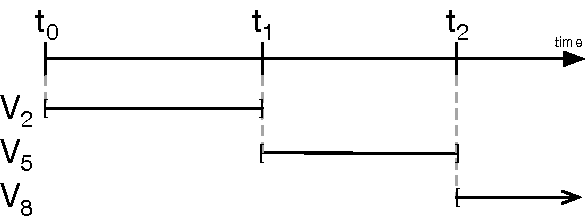
\includegraphics[width=0.5\linewidth]{img/chapt-tkm/validitySchemaC2}
%	\caption{Validity periods of the consumption values of one smart meters}
%	\label{fig:tkm:validityC2}
%\end{figure}

\begin{figure}
	\centering
	\subfloat[Consumption values] {
		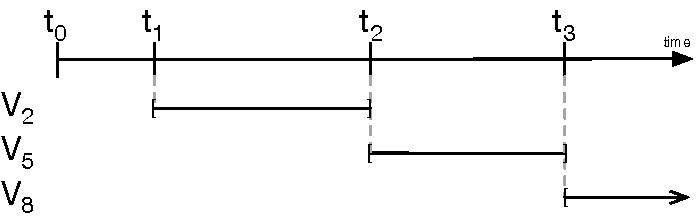
\includegraphics[width=0.4\linewidth]{img/chapt-tkm/formalism/validitySchemaC2}
		\label{fig:tkm:validityC2}
	}
	\hfil
	\subfloat[Edges]{
		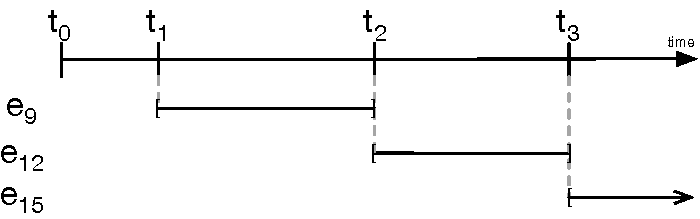
\includegraphics[width=0.4\linewidth]{img/chapt-tkm/formalism/validitySchemaC2Edges}
		\label{fig:tkm:validityC2Edges}
	}
	\caption{Validity periods of the consumptions values and their edges to the smart meter $M_2$}
\end{figure}

%More generally, the $V_{SG}^T$ returns:
%\begin{condItemize}
%	\item $\forall i \in [1..3], V^T_{SG}(V_i) = [t_0, t_1)$,
%	\item $\forall i \in [4..6], V^T_{SG}(V_i) = [t_1, t_2)$,
%	\item $\forall i \in [7..9], V^T_{SG}(V_i) = [t_2, t_\infty)$.
%\end{condItemize}
From these validity period, the $Z^T_{SG}$ can be used to navigate to the different values over time.
Let's continue with the same example, $C_2$.
In order to get the evolution of the consumption value $C_2$, given the initial one, one will use the $Z^T_{SG}$ relation:
\begin{itemize}
	\item $Z^T_{SG}(V_2, t_{s1}) = V_2$, where $t_0 \leqslant t_{s1} < t_1$
	\item $Z^T_{SG}(V_2, t_{s2}) = V_5$, where $t_1 \leqslant t_{s2} < t_2$
	\item $Z^T_{SG}(V_2, t_{s3}) = V_8$, where $t_2 \leqslant t_{s3} < t_\infty$.
\end{itemize}
%More generally, the $Z^T_{SG}$ returns:
%\begin{condItemize}
%	\item for $0 \leqslant t_s < t_1$:
%		\begin{condItemize}
%			\vspace{-0.5em}
%			\item $\forall i \in \{1, 4, 7\}, Z^T_{SG}(V_i, t_s) = V_1$,
%			\item $\forall i \in \{2, 5, 8\}, Z^T_{SG}(V_i, t_s) = V_2$,
%			\item $\forall i \in \{3, 6, 9\}, Z^T_{SG}(V_i, t_s) = V_3$.
%		\end{condItemize}
%	\vspace{-0.5em}
%	\item for $t_1 \leqslant t_s < t_2$:
%		\begin{condItemize}
%			\vspace{-0.5em}
%			\item $\forall i \in \{1, 4, 7\}, Z^T_{SG}(V_i, t_s) = V_4$,
%			\item $\forall i \in \{2, 5, 8\}, Z^T_{SG}(V_i, t_s) = V_5$,
%			\item $\forall i \in \{3, 6, 9\}, Z^T_{SG}(V_i, t_s) = V_6$.
%		\end{condItemize}
%	\vspace{-0.5em}
%	\item for $t_2 \leqslant t_s < t_\infty$:
%		\begin{condItemize}
%			\vspace{-0.5em}
%			\item $\forall i \in \{1, 4, 7\}, Z^T_{SG}(V_i, t_s) = V_7$,
%			\item $\forall i \in \{2, 5, 8\}, Z^T_{SG}(V_i, t_s) = V_8$,
%			\item $\forall i \in \{3, 6, 9\}, Z^T_{SG}(V_i, t_s) = V_9$.
%		\end{condItemize}
%\end{condItemize}



\paragraph{Description of \pmb{$E_{SG}$}}

In this example, edges are used to store the relationships between the different context elements.
For example, the edge between the substation $S_1$ and the fuse $F_1$ allow to represent the fact that the fuse is physically inside the substation.
Another example, edges between the cable $C_1$ and the meters $M_1$, $M_2$ and $M_3$ represent the fact that these meters are connected to the smart grid through this cable.

One may consider that relations (validity, $Z^T$, decisions, action processes and requirements processes) will be stored as edges.
But, this decision is let to the implementation part of this formalism.

In our model, only consumption values ($V_i$ nodes) are modified.
Plus, since the scenario do not imply other edges modifications, only those between meters and values are modified.
The edge set contains thus sixteen edges: $E_{SG} = \{E_i \mid i \in [1..16] \}$.

By definition, the unmodified edges have a validity period starting from $t_0$ and never ends: $\forall i \in [1..7], V^T_{SG}(E_i) = [t_0, t\infty)$.
The history of the three knowledge elements that represent consumption values do not only impact the nodes which represent the values but also the edges between those nodes and the meters ones:
\begin{itemize}
	\item $C_1$ impacts edges between $M_1$ and $V_1$, $V_4$, and $V_7$, \ie $\{E_8, E_{11}, E_{14}\}$,
	\item $C_2$ impacts edges between $M_2$ and $V_2$, $V_5$, and $V_8$, \ie $\{E_9, E_{12}, E_{15}\}$,
	\item $C_3$ impacts edges between $M_3$ and $V_3$, $V_6$, and $V_9$, \ie $\{E_{10}, E_{13}, E_{16}\}$.
\end{itemize}

Continuing with $C_2$ as example, the initial edge value is $E_8$ from $t_0$, which is replaced by $E_{11}$ from $t_1$, itself replaced by $E_{14}$ from $t_2$.
The validity relation, applied on these edges, thus returns:
\begin{itemize}
	\item $V^T_{SG}(E_8) = [t_0, t_1) = V^T_{SG}(V_2)$,
	\item $V^T_{SG}(E_{11}) = [t_1, t_2) = V^T_{SG}(V_5)$,
	\item $V^T_{SG}(E_{14}) = [t_2, t_\infty) = V^T_{SG}(V_8)$,
\end{itemize}

These validity periods are depicted in Figure~\ref{fig:tkm:validityC2Edges}.
As they are driven by those of consumption values ($V_2$, $V_5$, and $V_8$), they are equals.

As for nodes, the $Z^T_{SG}$ relation can navigate over time through these values.
For example, to get the history of the edges between the consumption value $C_2$ and the meter represented by $M_2$, one can apply the $Z^T_{SG}$ relation as following:
\begin{itemize}
	\item $Z^T_{SG}(E_8, t_{s1}) = E_8$, where $t_0 \leqslant t_{s1} < t_1$,
	\item $Z^T_{SG}(E_8, t_{s2}) = E_8$, where $t_1 \leqslant t_{s1} < t_2$,
	\item $Z^T_{SG}(E_8, t_{s3}) = E_8$, where $t_2 \leqslant t_{s1} < t_\infty$.
\end{itemize}


\paragraph{Description of \pmb{$R_{P_{SG}}$}}
The requirement calls for minimizing overloads.
It means that when the system detects at least one overload, for example in cables, it will take counter actions.
As the system has prediction capabilities, it will not only check is there is one at the current time $t$ but also if one will come in the next hour.
The pattern will be defined as follow: $P_{[t, t+15min]}$.
To determine if there is an overload, the system needs to know: the current and future consumption, the current and future topology.
The last one is used to compute the loads from the consumption (cf. Section~\ref{sec:intro:use-case}).

Let's consider that time points are regular and there is one every 15 minutes and that current time is $t_0$.
The pattern, $P_{[t_0, t_1]}$, will thus contain all nodes that are valid between $t_0$ and $t_1$ (included):
\begin{itemize}
	\item all topology nodes between: $\{S_1, C_1, F_1, F_2, D_{C_1}, M_1, M_2, M_3\}$
	\item all consumption values between: $\{V_i \mid i \in [1..6]\}$,
	\item all edges that connected these nodes: $\{E_i \mid i \in [1..13]\}$
\end{itemize}

From these values, the loads is computed and the system checks that none will exceed the capacity of the infrastructure (cables, substations, cabinets).

\paragraph{Description of \pmb{$A_{P_{SG}}$}}
Now, let us assume that the execution of $R_{P_{SG}}$ detects an overload on the cable ($C_1$) at $t_0$.
The system decides to reduce the amps limits, and thus the load, on the three meters.
The action $A_1$ (decreasing amps limits) is thus executed three times: one time per meter.
For each of these action, the input context will correspond to the pattern used by the requirement relation: $P_{[t_0, t_1]}$.
The output context will contain the predicted values after the actions have been executed.
Here, the actions are executed in parallel and their execution time is in seconds.
So the impact will be visible from $t_1$.
So the output pattern contain the three values at $t_1$:  $P_{[t_1, t_1]}$.
In summary:
\begin{itemize}
	\item Action 1: $A_{P_1}: P_{[t_0, t_1]} \rightarrow P_{[t_1, t_1]}$,
	\item Action 1: $A_{P_2}: P_{[t_0, t_1]} \rightarrow P_{[t_1, t_1]}$,
	\item Action 1: $A_{P_3}: P_{[t_0, t_1]} \rightarrow P_{[t_1, t_1]}$.
\end{itemize}


\paragraph{Description of \pmb{$D_{SG}$}}
Following the scenario, there is one decision, $D_{SG_1}$, which try to achieve the requirement $R_1$ by executing the actions $A_1$: $A_{P_1}$, $A_{P_2}$, and $A_{P_3}$.
Then, here the decision is equals to: $D_{SG_1} = \{R_1, A_{P_1}, A_{P_2}, A_{P_3}\}$.

\paragraph{Summrarize}
Through this section, I explifyed how the formalism can be used to define an adaptation decision on a smart grid system.
As the decision contains information about the circumstances and the impact, one may use it to debug the process and/or try to explain the behavior of such systems.